\documentclass[10pt, UKenglish, xcolor=svgnames]{beamer}
\usepackage{babel}
\usepackage[utf8]{inputenc}  
\usepackage{geometry}
\usepackage[customcolors]{hf-tikz}
\usepackage[T1]{fontenc}   
%\usepackage{tcolorbox}
\usepackage{siunitx}
\usepackage{graphicx}
\usepackage{hyperref}
\hypersetup{
    colorlinks=true,
    linkcolor=blue,
    urlcolor=cyan,
}
\usepackage{bookmark}
\usepackage{marvosym}
\usepackage{tikz}
\usepackage{tikz-qtree}
\usepackage{cancel}
\usepackage{todonotes}
\useoutertheme[subsection=false]{smoothbars}
\DeclareSIUnit[number-unit-product = {}]{\inchQ}{\textquotedbl}
\usepackage{amsmath,bm}
\DeclareSIUnit[number-unit-product = {\thinspace}]{\inch}{in}
\usetheme[menuwidth={0.3\paperwidth}]{erlangen}
\usepackage{multicol}
\usepackage{charter}
\setbeamercovered{transparent=20}
\setbeamertemplate{navigation symbols}{}
\sisetup{separate-uncertainty = true}
\usepackage[version=4]{mhchem}
\usepackage{tikz}
\usepackage{hepnames}
\usepackage{soul}
\usepackage{color}
\usepackage{thesis_defs}
\usepackage{subcaption}
\captionsetup[subfigure]{labelformat=empty}
\usepackage{xcolor}

% Use listings inside tcolorbox for listings
\usepackage[listings]{tcolorbox}
\tcbset{colframe=Blue, colback=Azure}
\tcbset{listing options={style=tcblatex,
  basicstyle=\ttfamily\scriptsize,
  keywordstyle=\color{blue},
  identifierstyle=\color{magenta}
}}


\usepackage[backend=biber]{biblatex}
\bibliography{bibliography.bib}

\graphicspath{%
  {./feynman_diagrams/}%
  {./figures_theory/}%
  {./figures_simple/}%
  {./figures_misc/}%
  {./app1/}%
  {./app2/}%
  {./app3/}%
}


\definecolor{color1}{RGB}{33,217,217}
\definecolor{color2}{RGB}{7,61,111}

\newcommand{\lr}{\mathcal{lr}}


\newcounter{totavalue}
\newcounter{parvalue}

\def\aux{1}
\def\radius{9pt}
\def\step{4pt}
\usepackage[absolute,overlay]{textpos}


\newcommand\circcounter{%
\ifnum\inserttotalframenumber<2\relax
\else
  \setcounter{totavalue}{\inserttotalframenumber}
  \setcounter{parvalue}{\insertframenumber}
  \ifnum\inserttotalframenumber>45\relax
    \renewcommand\step{0pt}
  \fi%
  \pgfmathsetmacro{\aux}{360/27}
  \begin{tikzpicture}[remember picture,overlay, rotate=90+\aux]
  \foreach \i in {0,1,...,27}
    \fill[logo_blue] 
      (0,0) -- (-\i*\aux:\radius) arc  (-\i*\aux:-(\i+1)*\aux+\step:\radius) -- cycle;
  \foreach \i in {1,...,\insertframenumber}
    \fill[logo_grey] 
      (0,0) -- (-\i*\aux:\radius) arc  (-\i*\aux:-(\i+1)*\aux+\step:\radius) -- cycle;
  \fill[white] circle (\radius/1.3);
  \node at (0,0) {\small\insertframenumber}; 
  \end{tikzpicture}%
\fi%
}


\usepackage{eso-pic,picture}



\begin{document} 

\title[]{Jet validation and other stories\\Qualification task report}
\subtitle{\today}
\author{Christian Kirfel}
%\institute{Universtität Bonn}
        



\begin{frame}[plain]
\vspace{0.0cm}
  \titlepage
      \AddToShipoutPictureFG*{%
    \AtPageUpperLeft{%
      \put(8.7cm,-9.6cm){

\includegraphics[scale=0.03]{original_logo.jpg}
\makebox(0,0)[lt]{}%
      }%
    }%
  }%
    \AddToShipoutPictureFG*{%
    \AtPageUpperLeft{%
      \put(0.0cm,-9.6cm){
%\includegraphics[scale=0.17]{atlas_gay.png}
%
\includegraphics[scale=0.17]{ATLAS-Logo-Ref-RGB-H_0.jpg}
\makebox(0,0)[lt]{}%
      }%
    }%
  }%
\end{frame}
\addtobeamertemplate{navigation symbols}{\vspace*{0.8cm}\hfill\circcounter\hspace*{0.7cm}}


\begin{frame}{General ML selection}
  \begin{columns}
    \begin{column}{0.5\textwidth}
      \centering 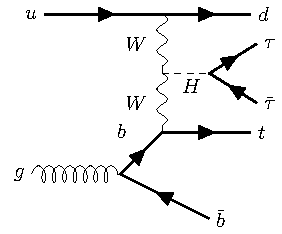
\includegraphics[width=0.45\textwidth]{/cephfs/user/s6chkirf/feynman_diagrams/tHq_tautau}\\
      \includegraphics[width=0.45\textwidth]{/cephfs/user/s6chkirf/feynman_diagrams/tHq_WW}
      \includegraphics[width=0.45\textwidth]{/cephfs/user/s6chkirf/feynman_diagrams/tHq_ZZ}
      \begin{itemize}
        \item n-jets: 2 (b-jets: \textbf{1})
        \item b-jet WP: 70 DL1r
        \item nLeptons \& nTaus: \bf{$1e / \mu~2\tau_{\text{had}}$}
        \item $E_{\text{T,miss}}$: no cut (to \SI{800}{GeV})
      \end{itemize}
    \end{column}
    \begin{column}{0.7\textwidth}
      \vspace*{-0.05\textwidth}
      \begin{itemize}
        \footnotesize
        \item jets:
        \vspace*{-0.02\textwidth}
        \begin{itemize}
          \footnotesize
          \item $p_T>\SI{35}{GeV}$
          \item $|\eta|<4.5$
          \item EMPFlow
        \end{itemize}
        \item electrons:
        \vspace*{-0.02\textwidth}
        \begin{itemize}
          \footnotesize
          \item $p_T>\SI{20}{GeV}$ leading \SI{27}{GeV}
          \item $|\eta|<2.5$ not in 1.37 - 1.52
          \item WP: LooseAndBLayerLH ; \\isolation: no requirement
        \end{itemize}
        \item muons:
        \vspace*{-0.02\textwidth}
        \begin{itemize}
          \footnotesize
          \item $p_T>\SI{20}{GeV}$ leading \SI{27}{GeV}
          \item $0.01<|\eta|<2.5$
          \item WP: Loose ; isolation: no requirement
        \end{itemize}
        \item taus:
        \vspace*{-0.02\textwidth}
        \begin{itemize}
          \footnotesize
          \item $p_T>\SI{20}{GeV}$ leading \SI{27}{GeV}
          \item $|\eta|<2.5$ not in 1.37 - 1.52
          \item WP: RNNLoose
          \item ASG recommended OLR ($\tau_{had}$ remove jets)
        \end{itemize}
      \end{itemize}
    \end{column}
  \end{columns}
\end{frame}
  

\section{Framework}
\begin{frame}
    \centering \Huge Work on the framework
\end{frame}

\begin{frame}{Technical work on the JetValidation}
    \begin{itemize}
        \item \href{https://gitlab.cern.ch/atlas/athena/-/merge_requests/40475}{Merge Request}
    \end{itemize}
    \begin{block}{JetSubstructureHistos}
        \begin{itemize}
            \item Class to manually calculate variables
            \item Tau21, Tau32, Tau21\_wta, Tau32\_wta, C1, C2, D2
        \end{itemize}
    \end{block}
    \begin{block}{Clearance}
        \begin{itemize}
            \item Removed empty histograms
            \item Rearranged according to new collections
        \end{itemize}
    \end{block}
    \begin{block}{AntiKt4EMPFlow}
        \begin{itemize}
            \item Added: DFCommonJets\_QGTagger\_NTracks, DFCommonJets\_QGTagger\_TracksWidth, DFCommonJets\_QGTagger\_TracksC1, DFCommonJets\_fJvt
        \end{itemize}
    \end{block}    
\end{frame}

\begin{frame}{Example of an added variable}
    \centering 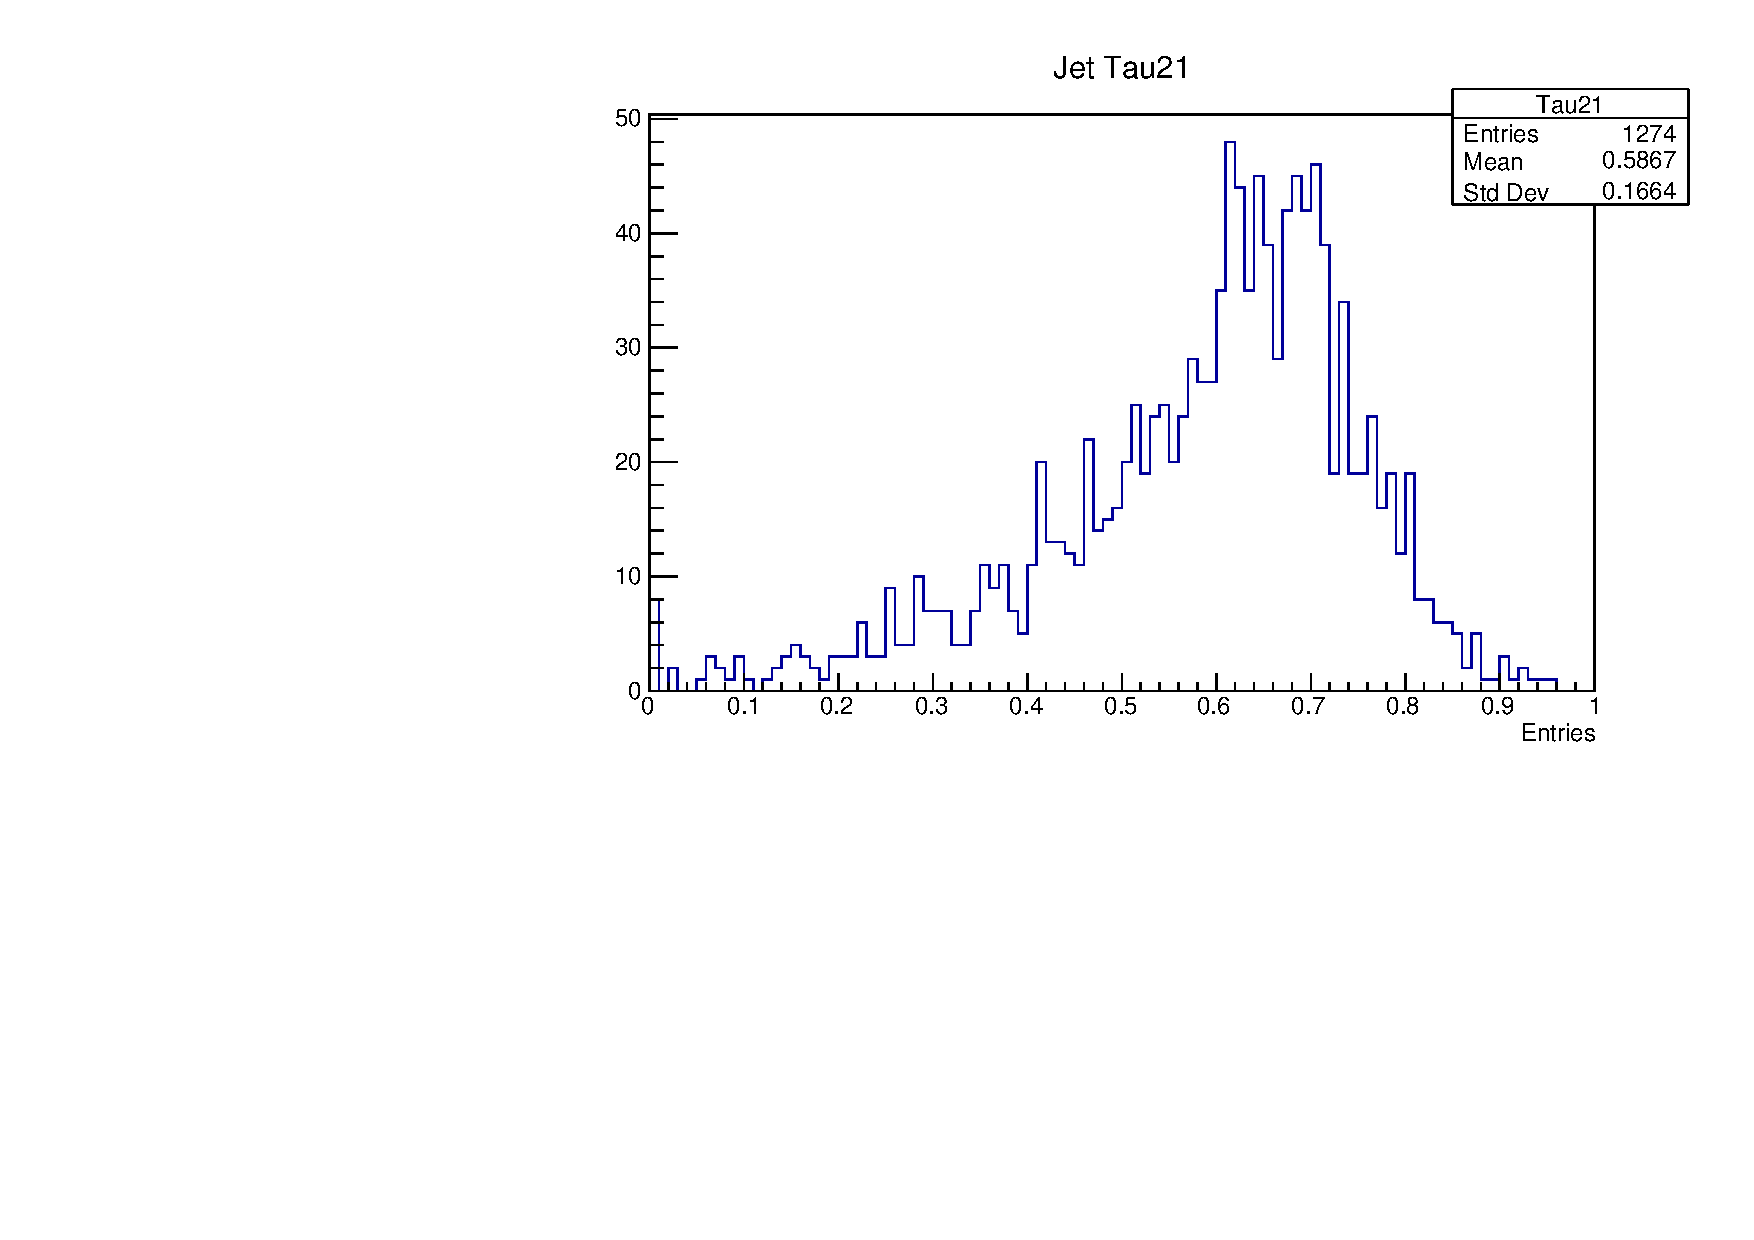
\includegraphics[width=\textwidth]{Tau21_example}
\end{frame}

\section{Validation}
\begin{frame}
    \centering \Huge Jet validation \\ An introduction
\end{frame}

\begin{frame}{What is validation}
    \begin{itemize}
        \item Necessary to make sure that the switch to r22 is correctly done
        \item Starting point were representative r21 MC samples for each group
        \item Format: Events to Hits to AOD to DAOD\_PHYSVAL to NTUP\_PHYSVAL
        \item NTUP\_PHYSVAL is just a histogram format useful for comparison
        \item Downloaded and overlaid plots are being created, evaluated and investigated
    \end{itemize}
\end{frame}

\begin{frame}{An example}
    \begin{itemize}
        \item Validation of jet reconstruction using FlowElements instead of PFO for release 22
        \item Sample: JZ7 
        \item Collections: AntiKt4EMPFlowJets, AntiKt4EMPFlowFEJets
    \end{itemize}
    \begin{figure}
        \centering
        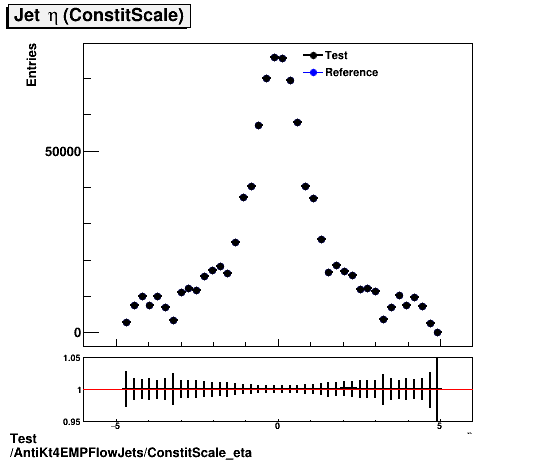
\includegraphics[width=0.64\textwidth]{goodAgreement.png}
    \end{figure}    
\end{frame}

\begin{frame}{Red plots}
    \begin{columns}
        \begin{column}{0.5\textwidth}
            \centering 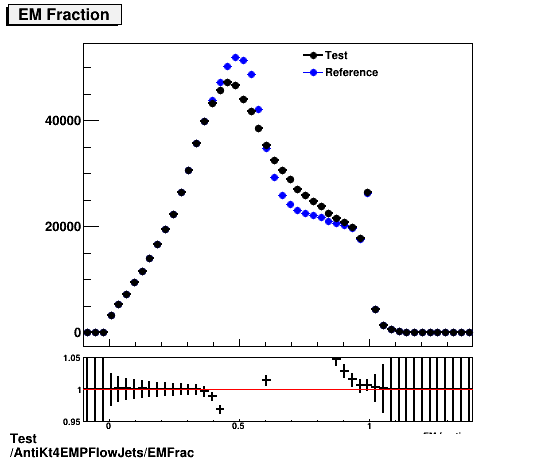
\includegraphics[width=0.72\textwidth]{FEEM}
            \centering 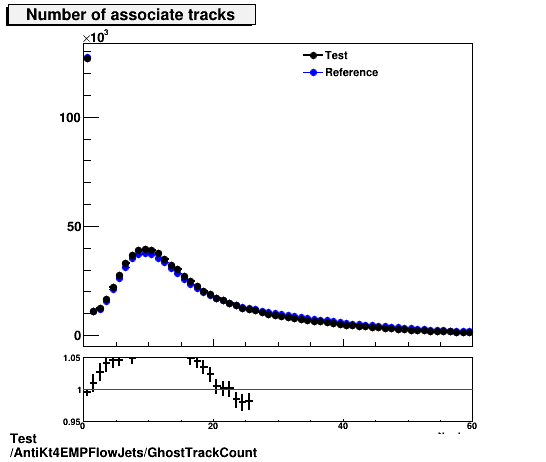
\includegraphics[width=0.72\textwidth]{FEtracks}
        \end{column}
        \begin{column}{0.5\textwidth}
            \centering 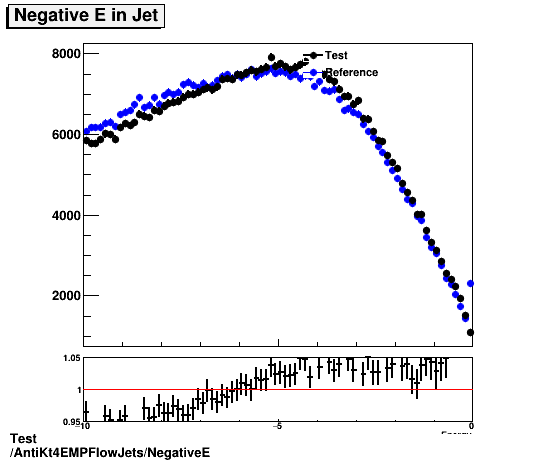
\includegraphics[width=0.72\textwidth]{FEnegE}
            \begin{itemize}
                \item Electromagnetic fraction, negative energy and number of associated tracks show bad agreement.
                \item The reason now has to be investigated
            \end{itemize}
        \end{column}
    \end{columns}
\end{frame}

\begin{frame}{Explanation of the disagreements}
    \begin{block}{Negative energy}
        Explained by the compression of topocluster moments in the AOD. Turning this off leads to perfect agreement.
    \end{block}
    \begin{block}{Number of associated tracks}
        Thinning applied at AOD level leads to TRT hits not being stored. Therefor PFlow had more tracks.
    \end{block}
    \begin{block}{Electromagnetic fraction}
        For very high energy deposits in EMB2 a default value was chosen for PFO.
    \end{block}
\end{frame}


\section{Tutorial}
\begin{frame}
    \centering \href{https://twiki.cern.ch/twiki/bin/viewauth/AtlasProtected/JsvJetPhysicsValidation}{\Huge A tutorial to validation}
\end{frame}

\begin{frame}{Producing validation plots}
    \begin{block}{Why would you need any of this?}
        \begin{itemize}
            \item You want to make plots for validation
            \item You want a nice tool to easily make comparison plots from ntuples
            \item It is actually quite easy!
        \end{itemize}
    \end{block}
    \begin{block}{What are the requirements}
        \begin{itemize}
            \item A grid certificate (if you want to download files via rucio)
            \item Access to athena
            \item A gitlab account
        \end{itemize}
    \end{block}
\end{frame}
%
\begin{frame}{An example task}
   \begin{itemize}
       \item The details of the task are unimportant
       \item It shows good behaviour for an example
   \end{itemize}
   \begin{block}{Details of the task}
       \begin{itemize}
           \item Description: Validation of G4fix quasi-stable particle simulation for Run2 re-processing
           \item JIRA: https://its.cern.ch/jira/browse/ATLPHYSVAL-701
           \item Reference: valid1:valid1.410000.PowhegPythiaEvtGen\_P2012\_ttbar\_hdamp172p5\_nonallhad.merge.NTUP\_PHYSVAL.e4993\_s3634\_r12287\_p4360\_p3821
           \item Test: valid1:valid1.410000.PowhegPythiaEvtGen\_P2012\_ttbar\_hdamp172p5\_nonallhad.merge.NTUP\_PHYSVAL.e4993\_s3227\_s3653\_r12320\_p4360\_p3821
           \item \href{https://atlas-computing.web.cern.ch/atlas-computing/links/PhysValDir/JetEtMiss/exampleValidation_CKIRFEL/}{Webpage}
       \end{itemize}
   \end{block} 
\end{frame}
%
\begin{frame}[containsverbatim]{Setup}
        \begin{tcblisting}{listing only}
git clone ssh://git@gitlab.cern.ch:7999/ckirfel/jetphysvalidation.git
cd jetphysvalidation            
setupATLAS
lsetup 'rucio -w'
voms-proxy-init -voms atlas
        \end{tcblisting}
    Set up rucio as wrapper to avoid polluting environment
    This works only for CLI and no rucio APIs available
\end{frame}
%
\begin{frame}[containsverbatim]{Getting the files}
    \begin{tcblisting}{listing only}
        ./JetVal.sh
    \end{tcblisting}
    \centering 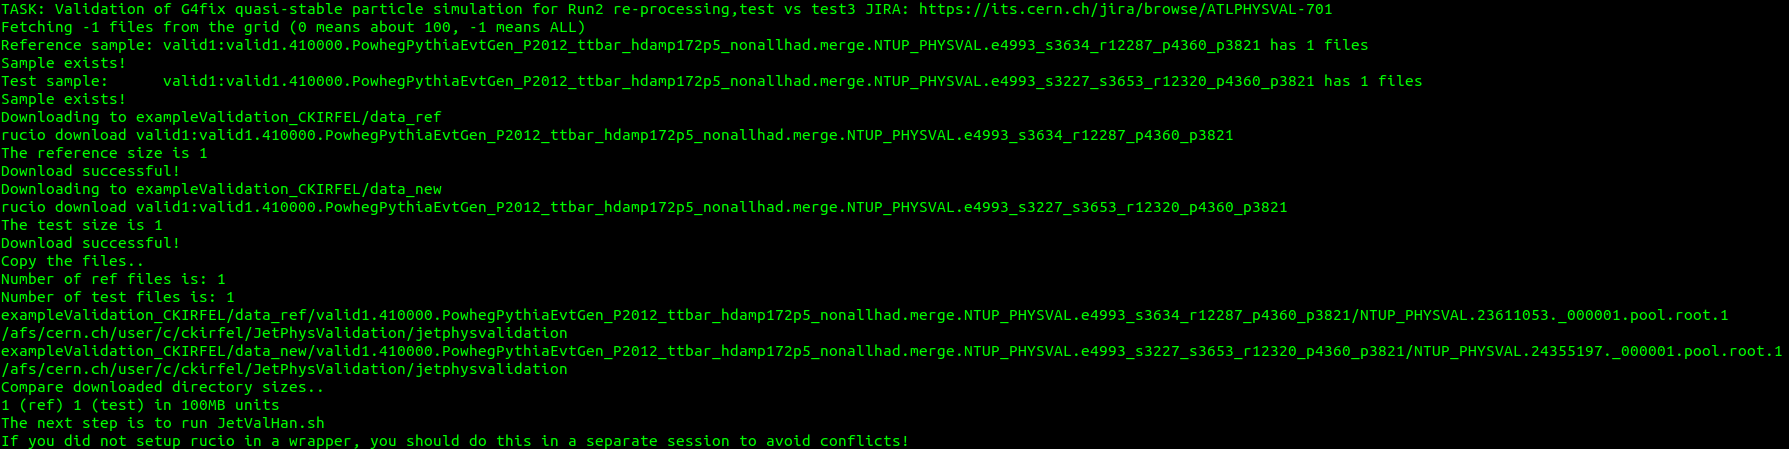
\includegraphics[width=\textwidth]{JetVal.png}    
\end{frame}
%
\begin{frame}[containsverbatim]{Making the comparison plots}
    \begin{tcblisting}{listing only}
        ./JetValHan.sh
    \end{tcblisting}
    \centering 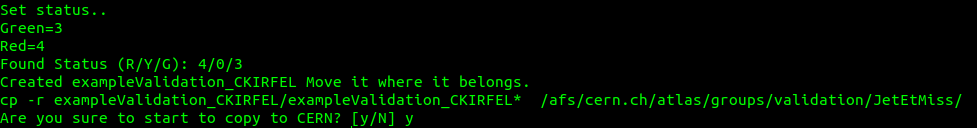
\includegraphics[width=\textwidth]{JetValHan.png}
\end{frame}
%
\begin{frame}{Checking the plots}
    \centering 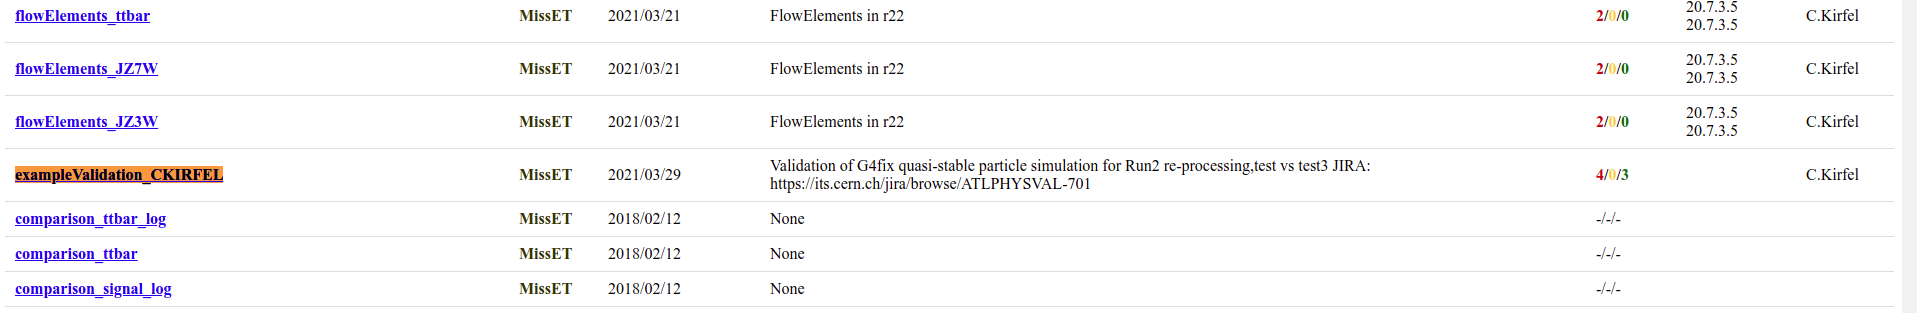
\includegraphics[width=\textwidth]{webpage.png}
    \href{https://atlas-computing.web.cern.ch/atlas-computing/links/PhysValDir/JetEtMiss/}{Validation webpage}
\end{frame}
%
\begin{frame}{Good agreement}
    \centering 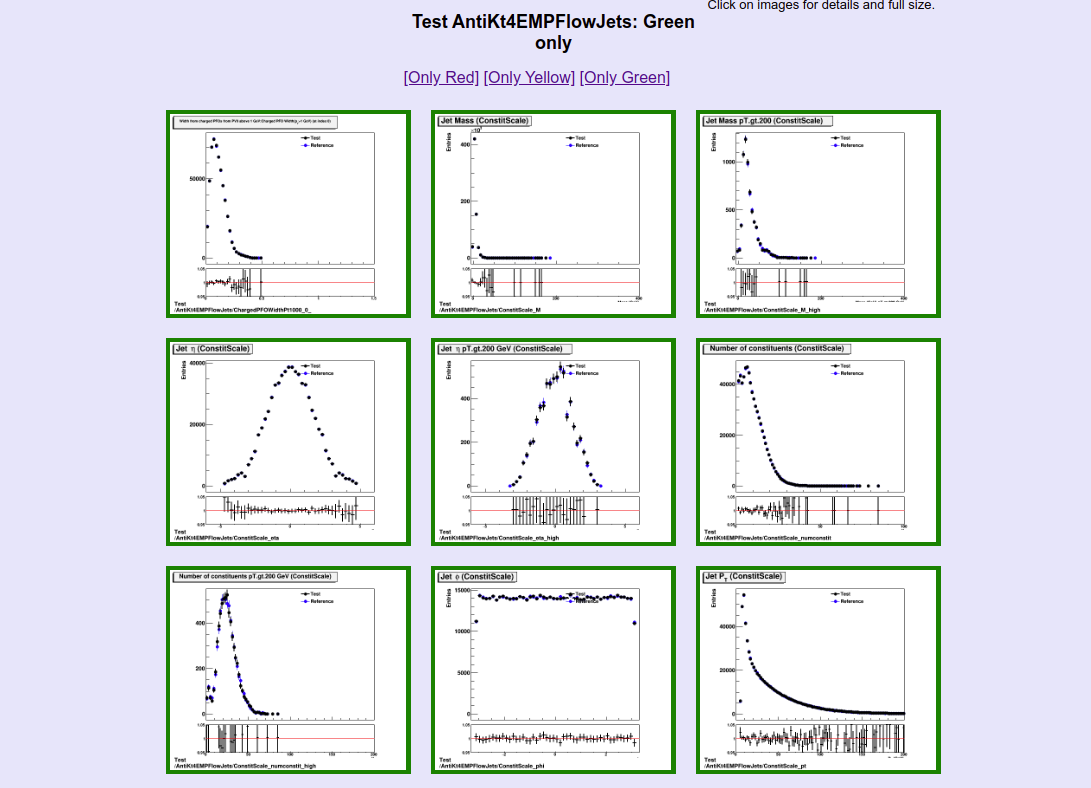
\includegraphics[width=\textwidth]{green.png}
\end{frame}
%
\begin{frame}{Medium agreement}
    \centering 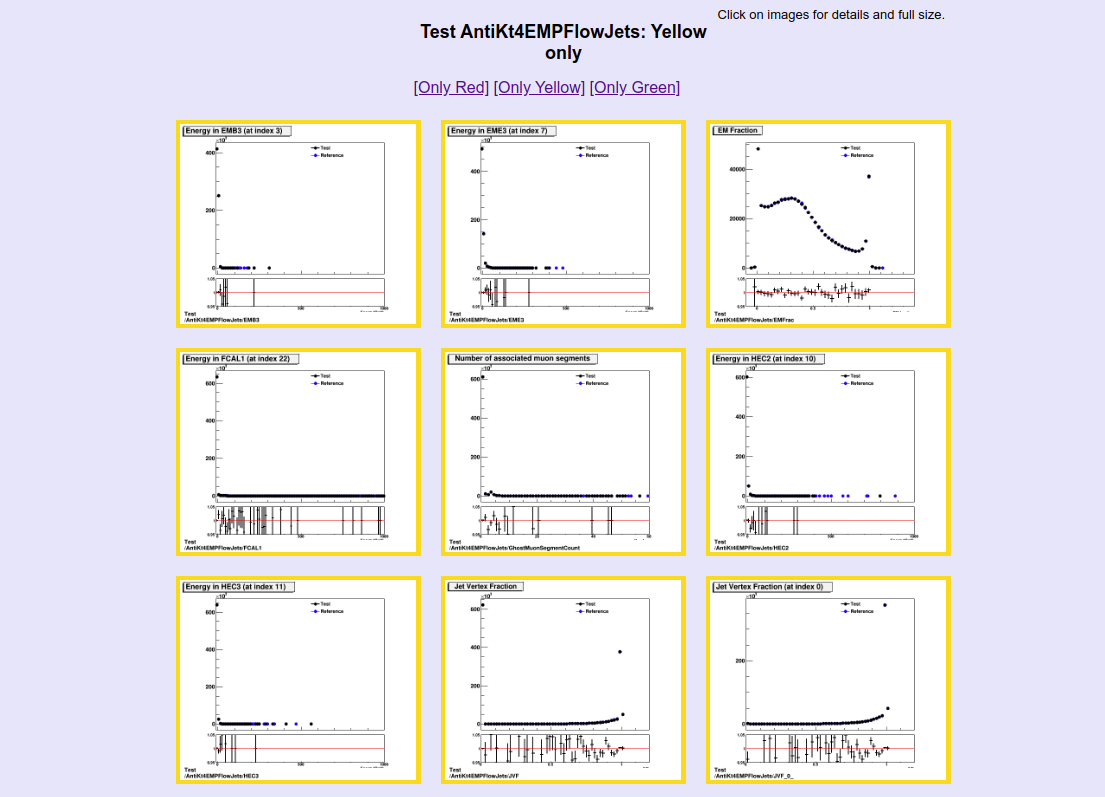
\includegraphics[width=\textwidth]{yellow.png}
\end{frame}
%
\begin{frame}{Bad agreement}
    \centering 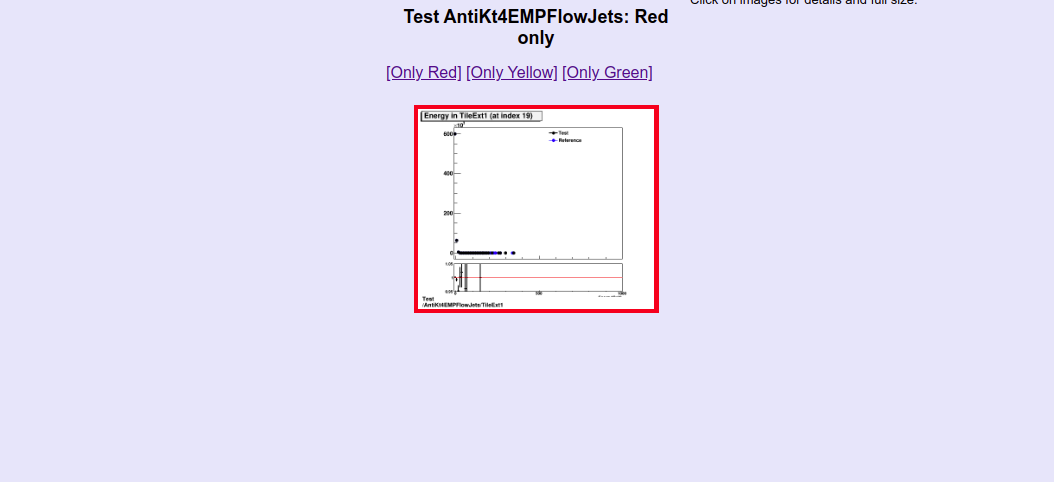
\includegraphics[width=\textwidth]{red.png}
\end{frame}
%
\begin{frame}{A plot in detail}
    \centering 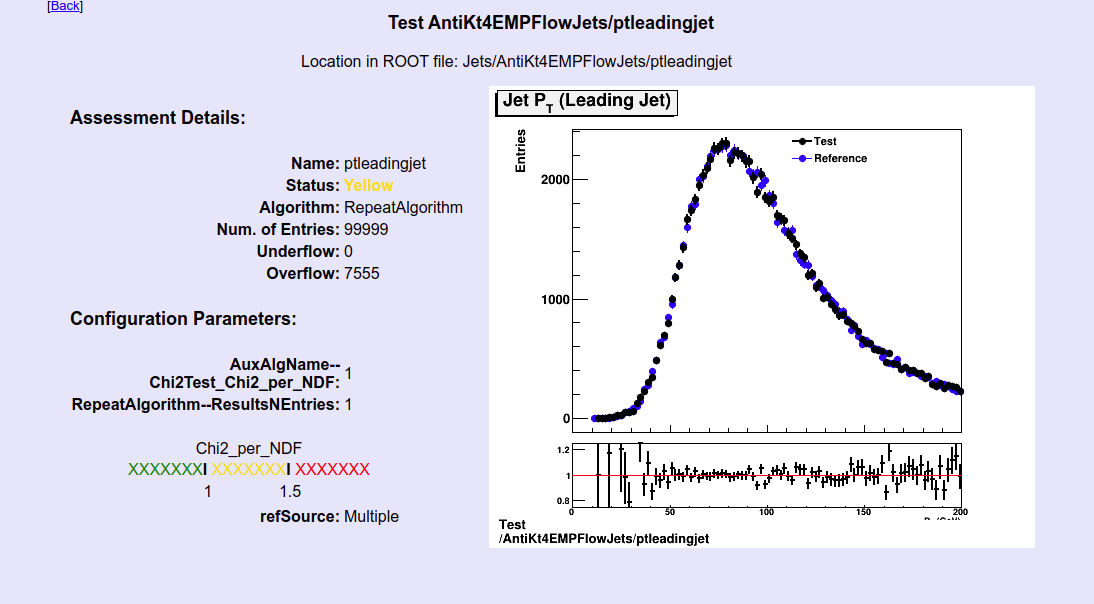
\includegraphics[width=\textwidth]{details.png}
\end{frame}
%
\begin{frame}{Checking the range}
    \centering 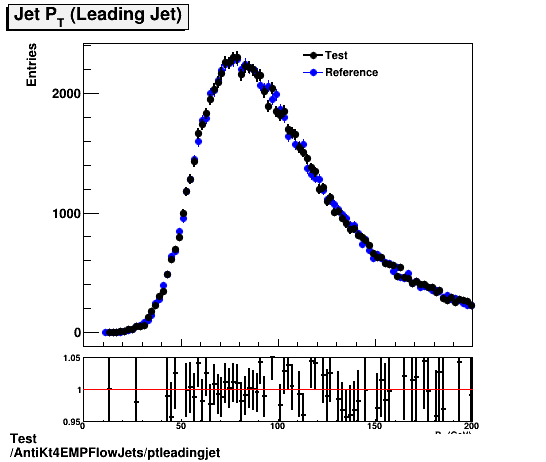
\includegraphics[width=0.7\textwidth]{smallRange.png}
\end{frame}
%
\begin{frame}{Checking the range}
    \centering 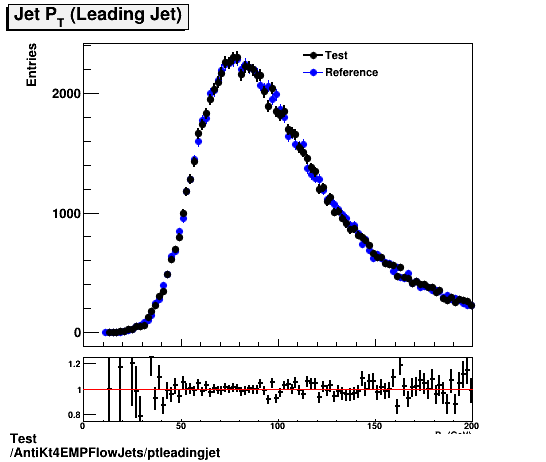
\includegraphics[width=0.7\textwidth]{largeRange.png}
\end{frame}

\begin{frame}[containsverbatim]{Utilized scripts 1: The web display}
    \begin{itemize}
        \item Tool to adjust the webdisplay
        \item Commonly used adjustments are arguments
        \item Some details have to be changed in the code
        \item \href{https://twiki.cern.ch/twiki/bin/viewauth/AtlasProtected/PhysValMonitoring}{TWiki}
    \end{itemize}
    \begin{tcblisting}{listing only}
        physval_make_web_display.py
        --reffile Reference:val_ref/output_ref.root 
        --outdir=$PROJECT --title Test val_new/output_new.root
        --startpath=Jets 
        --ratio --ratiorange=0.25 
        --normalize (or better scaleref)
    \end{tcblisting}
\end{frame}
%
\begin{frame}[containsverbatim]{Utilized scripts 2: The merger}
    \begin{itemize}
        \item Code used to merge multiple input files
    \end{itemize}
    \begin{tcblisting}{listing only}
        NTUPMerge_tf.py
        --inputNTUP_PHYSVALFile=$MERGE_REF 
        --AMITag="p3821" 
        --outputNTUP_PHYSVAL_MRGFile="output_ref.root"
    \end{tcblisting}
\end{frame}

%
\begin{frame}{Troubleshooting. Do not make my mistakes}
    \begin{itemize}
        \item You are using athena scripts, if you switched to a newer version that might have broken the code
        \item You might have used a local version of a script and forgot to switch back to the athena version
        \item Check that you have rights to push to the webpage
        \item You can always manually check that all files are in place and filled
        \item Check that you are not using the same file as test and ref by accident...
    \end{itemize}
\end{frame}
\begin{frame}{Conclusion and future steps}
    \begin{itemize}
        \item Both neural network and BDT show very good separation for an early stage of optimisation
        \vspace{0.2cm}
        \item For the lepditau channel the separation is outstanding but the stability is bad. This means the agreement between training and validation is often bad
        or has regions that are not understood.
        \vspace{0.2cm}
        \item In both cases the variables have a significant impact on the result. Different sets of features need to be explored to find better separations.
        \vspace{0.2cm}
        \item A decorrelation and ranking would be desireable
        \vspace{0.2cm}
        \item The handling of negative weights is an ongoing problem that needs to be investigated to see if a conclusion can be reached for MVA techniques.
    \end{itemize}
\end{frame}


\begin{frame}[plain,c]
%\frametitle{A first slide}

\begin{center}
\Huge Backup
\end{center}

\end{frame}

\begin{frame}{Evolutionary neural networks}
    \begin{itemize}
        \item Starting with a set of random configurations
        \vspace{0.2cm}
        \item Evaluate the results of the first generation and generate a new generation based on AUC 
        \vspace{0.2cm}
        \item Repeat until a good configuration is reached
        \vspace{0.2cm}
        \item Advantages:
            \begin{itemize}
                \item Decrease user bias for hyperparameter choice
                \item Optimised to run on worker nodes
                \item Quick discarding of bad configurations
                \item User friendly for unexperienced students
            \end{itemize}
    \end{itemize}
\end{frame}

%\begin{frame}{Inner product}
%    \begin{equation*}
%        a^{\mu} = \begin{pmatrix}
%            p_T \cosh ( \eta ) \\
%            p_T \cos ( \phi ) \\
%            p_T \sin ( \phi ) \\
%            p_T \sinh ( \eta ) \end{pmatrix}
%    \end{equation*}
%    %
%    \begin{align*}
%        \langle A | B \rangle = A_{\mu} B^{\mu}\\
%        = p_{T,A} p_{T,B} ( \cosh ( \eta_A ) \cosh ( \eta_B ) - \cos ( \phi_A ) \cos ( \phi_B)\\
%        - \sin ( \phi_A ) \sin ( \phi_B ) -\sinh ( \eta_A ) \sinh ( \eta_B ) )\\
%        = p_{T,A} p_{T,B} \left( \cosh ( \eta_A - \eta_B ) - \cos ( \phi_A - \phi_B ) \right)
%    \end{align*}
%\end{frame}

\begin{frame}{Responses}
  \begin{columns}
    \begin{column}{0.5\textwidth}
      \begin{figure}
      \centering 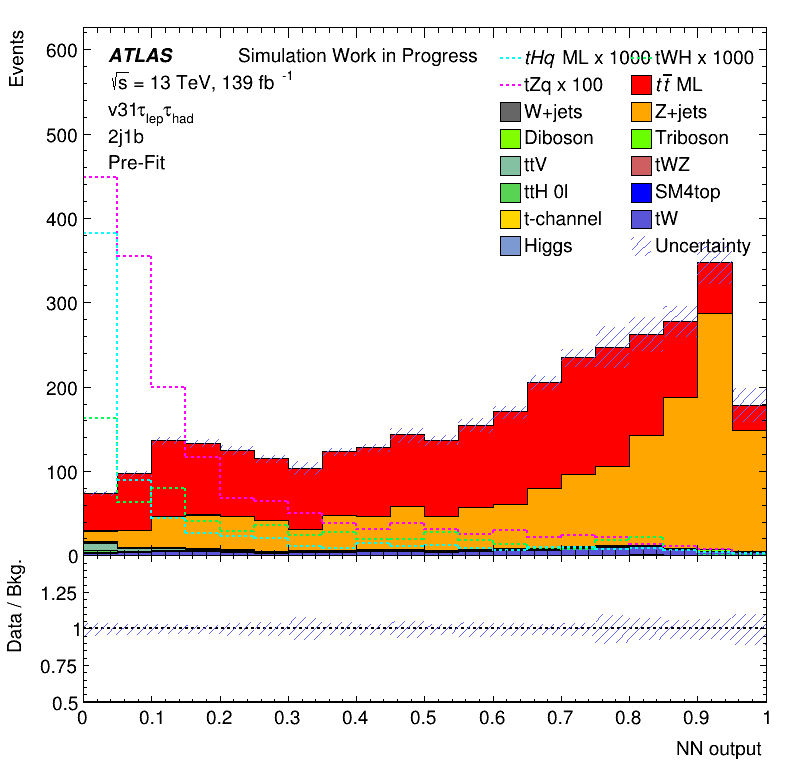
\includegraphics[width=\textwidth]{response_bkg}
      \caption{Background response}
      \end{figure}
    \end{column}
    \begin{column}{0.5\textwidth}
      \begin{figure}
      \centering 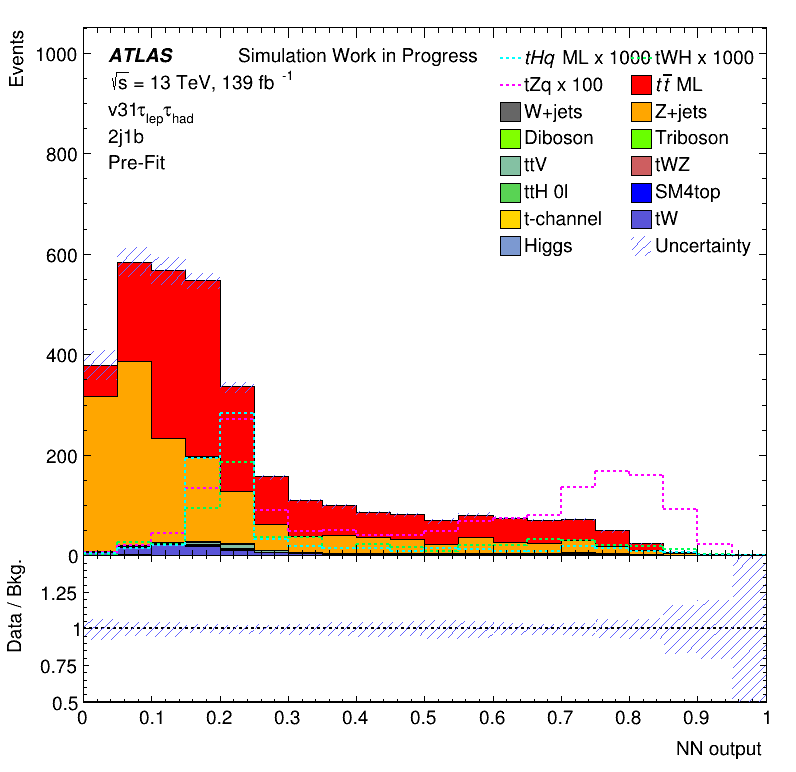
\includegraphics[width=\textwidth]{response_tZq}
      \caption{\tZq response}
      \end{figure}
    \end{column}
  \end{columns}
\end{frame}

\begin{frame}{\tHq versus \tZq}
  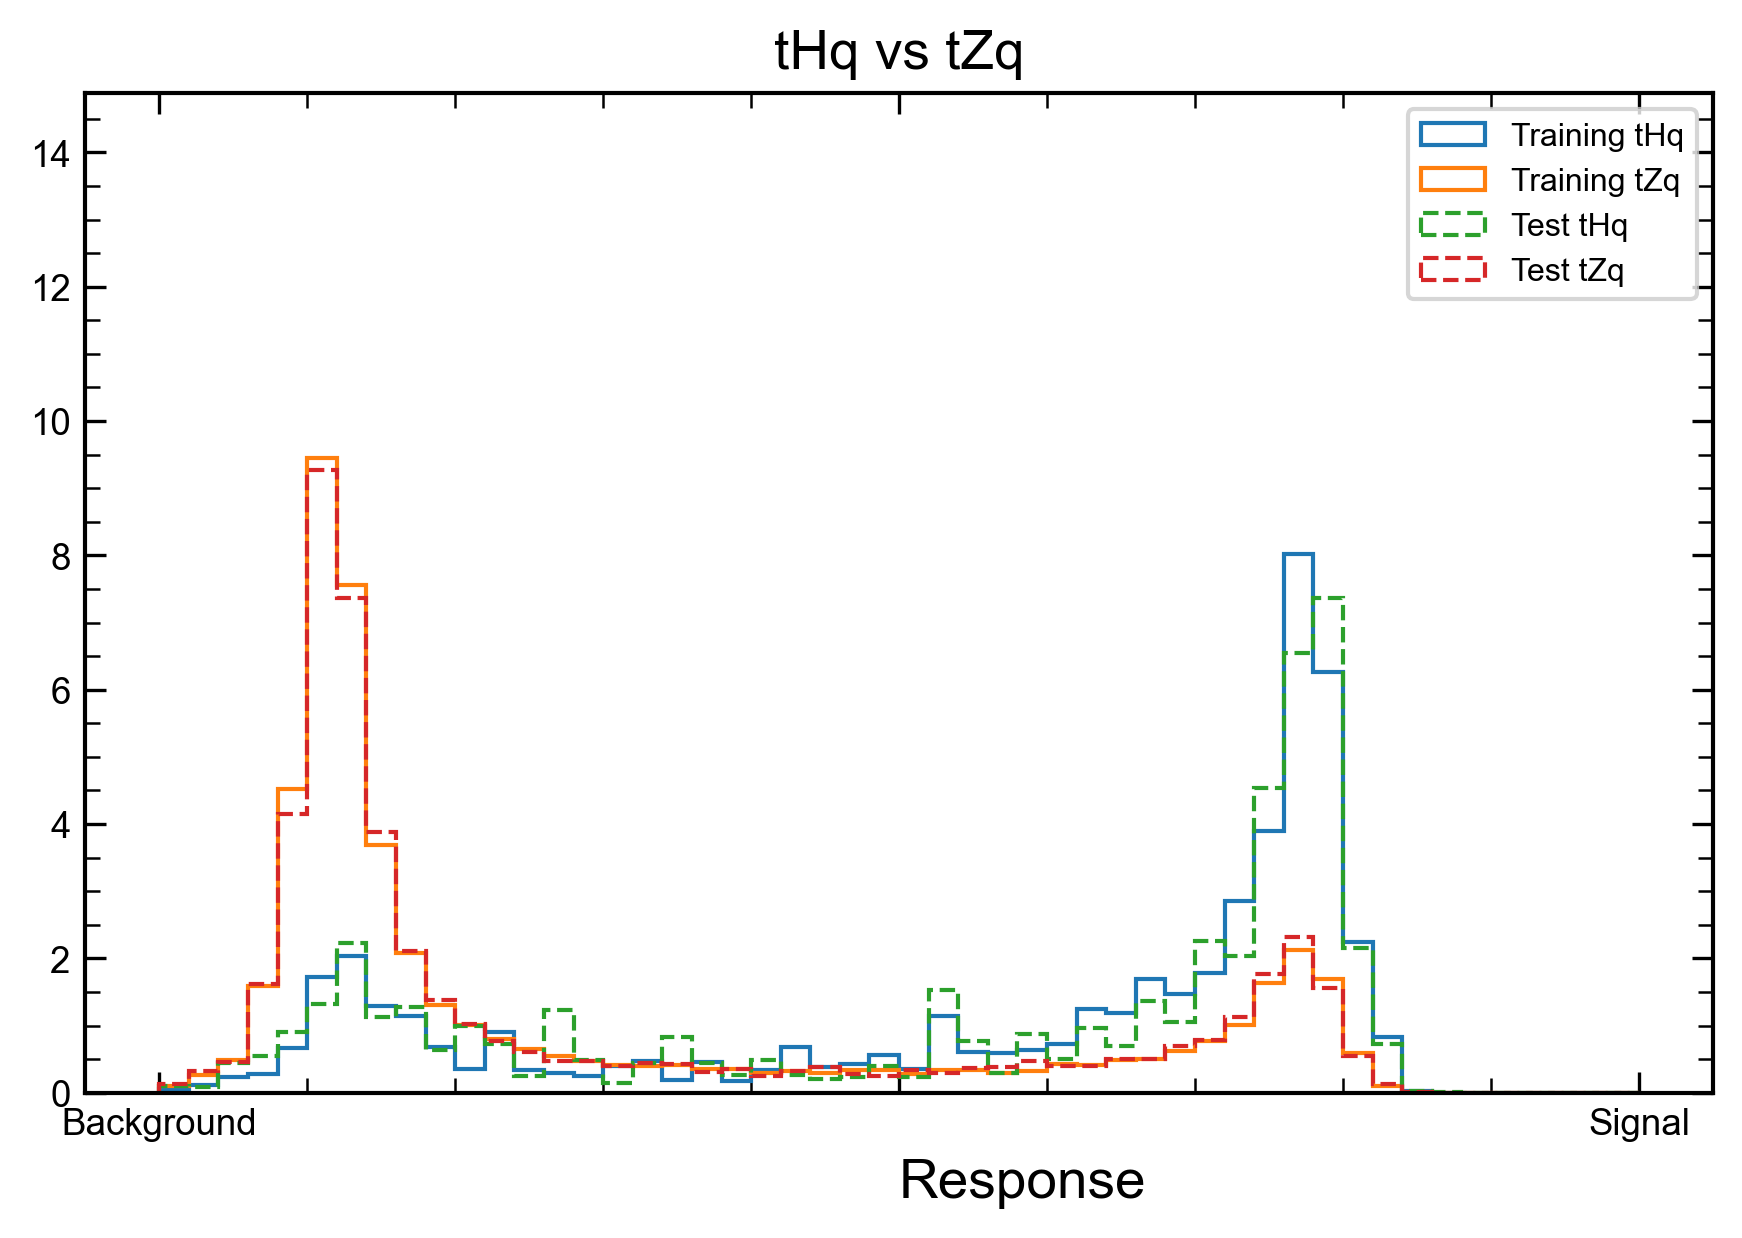
\includegraphics[width=\textwidth]{tHqvstZq.png}
\end{frame}

\begin{frame}{BDT summary}
    \begin{itemize}
        \item {\large A cut a bit below 0.2 would remove around 99\% of bkg
            events and 80\% of signal. Having just the 1\% of the bkg
            and 20\% of the signal would greatly increase our
            significance.}
        \vspace{0.2cm}
        \item {\large With the cut on the BDT we would have (approx.): bkg/sg = 4877/20 = 243
              Improved by a factor 71 to the before-presel scenario. Including BDT score in the trees}
        \vspace{0.2cm}
        \item {\large Using all events, not just the ones with positive weights reduces AUC surprisingly significantly}
        \vspace{0.2cm}
        \item {\large In the future the BDT should be tested in specific regions or for specific backgrounds}
    \end{itemize}
\end{frame}

\begin{frame}{}
  \centering 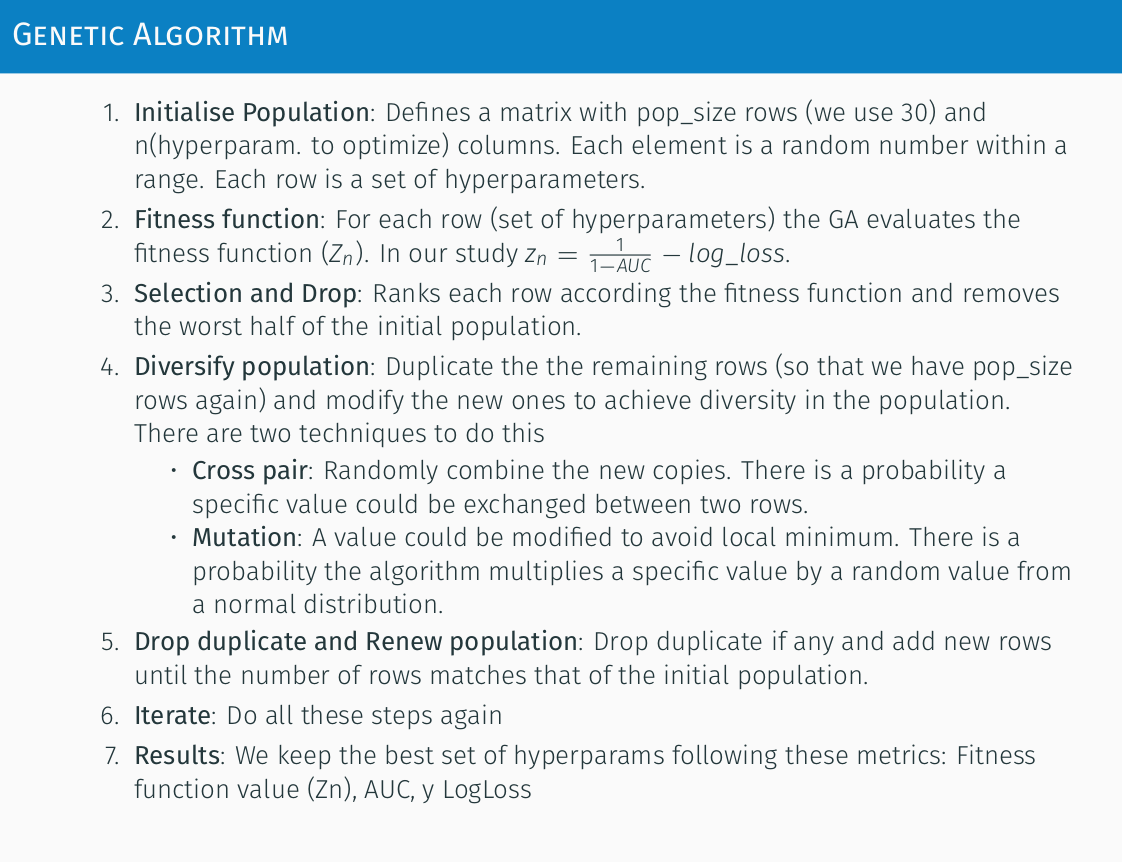
\includegraphics[width=\textwidth]{geneticAlg}
\end{frame}











\end{document}